%+++++++++++++++++++++++++++++++++++++++++++++++++++++++++++++++
% SUMMARY    : Vectors, Matricies, Distance and Norms 
%            : University of Southern Maine 
%            : @james.quinlan
%            : Ethan Gilles - Lecture 1
%+++++++++++++++++++++++++++++++++++++++++++++++++++++++++++++++
\section*{Objectives}
\begin{outline}
    \1 Introduction to Vectors
    \1 Distance Metrics
    \1 Distance Metric Examples
    \1 ``Homework" Problems
\end{outline}

\rule[0.0051in]{\textwidth}{0.00025in}
% ----------------------------------------------------------------

\section{Introduction to Vectors}

All vectors are part of a real space that has $p$ dimensions. We can show them using points in a Euclidean space.

\[
  \vec{x} \in \mathbb{R}^p
\] 

$p$ is always the number of \textbf{components} (number of elements) in a vector. For vectors with one component, $p$ would be equal to one. $p$ represents the dimension of space that vector is in.
\begin{center}
    
\begin{tikzpicture}[scale=0.7]
    \begin{scope}[xshift=0cm] 
        % 2D Point (p = 2)
        \begin{scope}[xshift=0cm] % Shift for 2D plot
            \draw[thick,->] (0,0) -- (4,0) node[anchor=north]{$x$};
            \draw[thick,->] (0,0) -- (0,4) node[anchor=east]{$y$};

            \coordinate (P2D) at (2,3);
            \draw[dashed] (P2D) -- (2,0) node[anchor=north]{};
            \draw[dashed] (P2D) -- (0,3) node[anchor=east]{};

            \filldraw[blue] (P2D) circle (2pt);

            \node[above right=5pt] at (P2D) {$p = 2$};
        \end{scope}

        % 3D Point (p = 3)
        \begin{scope}[xshift=6cm] % Shift for 3D plot
            \tdplotsetmaincoords{70}{110} % Set the viewing angles
            \begin{scope}[tdplot_main_coords]
                \draw[thick,->] (0,0,0) -- (4,0,0) node[anchor=north east]{$x$};
                \draw[thick,->] (0,0,0) -- (0,4,0) node[anchor=north west]{$y$};
                \draw[thick,->] (0,0,0) -- (0,0,4) node[anchor=south]{$z$};

                \coordinate (P3D) at (2,3,1);
                \draw[dashed] (P3D) -- (2,0,0) node[anchor=north]{};
                \draw[dashed] (P3D) -- (0,3,0) node[anchor=north]{};
                \draw[dashed] (P3D) -- (0,0,1) node[anchor=east]{};

                \filldraw[red] (P3D) circle (2pt);
                \node[above right=5pt] at (P3D) {$p = 3$};
            \end{scope}
        \end{scope}
    \end{scope}
\end{tikzpicture}
\end{center}

Vectors are notated like so:

% -- Column Major Vector
  \begin{align*}
    \vec{x} &= \begin{bmatrix}
           x_{1} \\
           x_{2} \\
           x_{3} \\
           \vdots \\
           x_{p}
         \end{bmatrix}
  \end{align*}

In the programming language you choose, make sure to know whether it is \textbf{Column Major} or \textbf{Row Major}. Almost all vectors will be shown in the \textbf{Column major} form.


Transposing a matrix will switch the matrix from column-major to row-major form or vice versa.
% -- Column Major Vector
  \begin{align*}
    x &= \begin{bmatrix}
           x_{1} \\
           x_{2} \\
            x_{3} \\
           \vdots \\
           x_{p}
         \end{bmatrix} \\
    x^T &= [\; x_1, \; x_2, \; x_3, \; \cdots \; x_p \;]
  \end{align*}



% ----------------------------------------------------------------
\section{Distance Metrics}
A \textbf{Distance Metric} is a general and abstract concept for the distances between vectors. They describe a function that takes two vectors and maps them to a real number greater than or equal to zero. 

\[
    d(x,y):= \vec{x} \times \vec{y} \rightarrow \mathbb{R}^+
\]

There are four conditions that a distance metric has to satisfy. To prove that a function on two vectors is a distance metric, show that these four statements are true for the function:

\begin{outline}
    \1 $d(x, y) \ge 0$. \; No negative values for distance
    \1 $d(x,y) = 0$ if $x = y$. \; Two of the same vectors should have 0 distance
    \1 $d(x,y) = d(y,x)$. \; The function must be symmetric and work with either order.
    \1 $d(x,z) \le d(x,y) + d(y,z)$. \; \textit{Triangle Inequality} shown below:
\end{outline}

\begin{center}
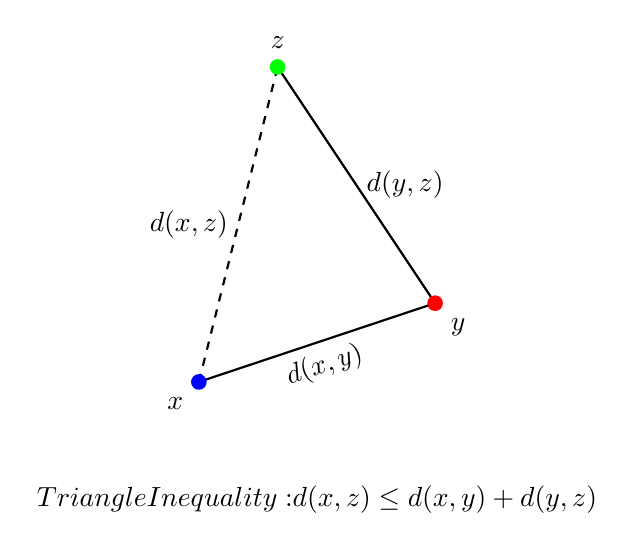
\begin{tikzpicture}
    \coordinate (x) at (0, 0);
    \coordinate (y) at (3, 1);
    \coordinate (z) at (1, 4);
    \draw[thick] (x) -- (y) node[midway, below, sloped] {$d(x, y)$};
    \draw[thick] (y) -- (z) node[midway, right] {$d(y, z)$};
    \draw[thick, dashed] (x) -- (z) node[midway, left] {$d(x, z)$};
    \node[circle, fill=blue, inner sep=2pt, label=below left:{$x$}] at (x) {};
    \node[circle, fill=red, inner sep=2pt, label=below right:{$y$}] at (y) {};
    \node[circle, fill=green, inner sep=2pt, label=above:{$z$}] at (z) {};
    \node at (1.5, -1.5) {$\text{Triangle Inequality: } d(x, z) \le d(x, y) + d(y, z)$};
\end{tikzpicture}
\end{center}

% ----------------------------------------------------------------
\section{Distance Metric Examples}

One of the distance metrics we all know of is \textbf{Euclidean Distance}, which is generally what we think of when the word \textit{distance} is used.

\begin{center}
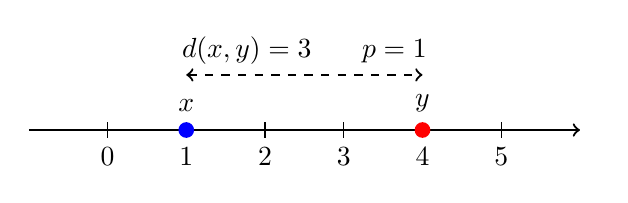
\begin{tikzpicture}
    \draw[->, thick] (-1, 0) -- (6, 0) node[right] {};
    \foreach \x in {0, 1, 2, 3, 4, 5}
        \draw (\x, 0.1) -- (\x, -0.1) node[below] {$\x$};
    \node[circle, fill=blue, inner sep=2pt, label=above:{$x$}] (A) at (1, 0) {};
    \node[circle, fill=red, inner sep=2pt, label=above:{$y$}] (B) at (4, 0) {};
    \draw[<->, thick, dashed] (1, 0.7) -- (4, 0.7) node[midway, above] {$d(x, y) = 3$ \; \; \;$p = 1$};
\end{tikzpicture} \\
Where $d(x,y) = |x - y|$ and $d(x, y)$ is the distance metric.
\end{center}

\begin{center}

    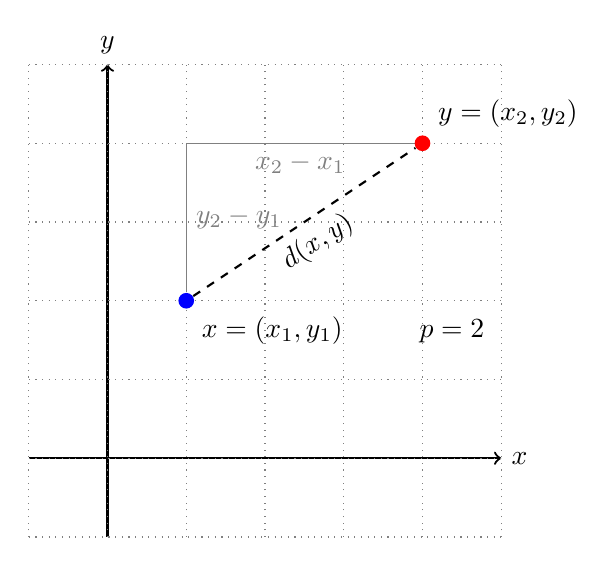
\begin{tikzpicture}
        \draw[->, thick] (-1, 0) -- (5, 0) node[right] {$x$};
        \draw[->, thick] (0, -1) -- (0, 5) node[above] {$y$};
        \draw[gray, dotted] (-1, -1) grid (5, 5);
    
        % Points A and B
        \node[circle, fill=blue, inner sep=2pt, label= below right:{$x = (x_1, y_1)$ \; \; \; \; $p = 2$}] (A) at (1, 2) {};
        \node[circle, fill=red, inner sep=2pt, label=above right:{$y = (x_2, y_2)$}] (B) at (4, 4) {};
    
        % Draw the Euclidean distance between A and B
        \draw[thick, dashed] (A) -- (B) node[midway, below, sloped] {$d(x, y)$};
    
        % Draw horizontal and vertical lines to show the components of the distance
        \draw[thin, gray] (A) -- (A |- B) node[midway, right] {$y_2 - y_1$};
        \draw[thin, gray] (B) -- (A |- B) node[midway, below] {$x_2 - x_1$};
    \end{tikzpicture} \\
Where $d(x,y) = \sqrt{(x_1 - y_1)^2 + (x_2 - y_2)^2}$
\end{center}

The Euclidean distance is one example of a metric used to define distance; however, there are many metrics used to define distances between vectors. \\

Another example of a distance metric is the \textbf{Hamming Distance}. The value of the Hamming Distance is found by counting the number of components that are not the same in two vectors. The Hamming distance is denoted by $d_H (x,y)$. For example:

\[
d_H \left( \mathbf{x} = 
\begin{bmatrix}
    1 \\
    3 \\
    4 \\
    7
\end{bmatrix}, 
\quad
\mathbf{y} = 
\begin{bmatrix}
    1 \\
    6 \\
    4 \\
    9
\end{bmatrix} \right) = 2
\quad \quad \quad 
d_H \left( \mathbf{x} = 
\begin{bmatrix}
    2 \\
    3 \\
    8 \\
    7
\end{bmatrix},
\quad
\mathbf{y} = 
\begin{bmatrix}
    1 \\
    6 \\
    4 \\
    9
\end{bmatrix} \right) = 4
\]

The Hamming distance uses the \textbf{Binary Indicator Function} on each component in two vectors to determine the total distance. The binary indicator function takes two components and outputs 1 if they are different and 0 if they are equal.

\[
\mathcal{I}(x,y) = 
\begin{cases}
    1 & if \; x \neq y\\
    0 & if \; x = y
\end{cases}
\]

Using the \textbf{Binary Indicator Function} we can describe the \textbf{Hamming Distance}:

\[
    d_H(x,y):= \sum^p_{i=1} \mathcal{I}(x_i \, , \, y_i)
\]


% ----------------------------------------------------------------
\section{Exploration (XPL) Problems}

\begin{outline}[enumerate]

\1  Is $d(x,y) = \sqrt{|x| + |y|}$ a valid distance metric? \\

We can show this by confirming the 4 conditions of a distance metric:

(i) $d(x,y) \ge 0$: This is \textbf{true} as the range of the square root function is $[0,\infty)$.

(ii) $d(x,y) = 0$ if $x=y$. This is \textbf{not true}. If $x=y$, then we have $\sqrt{2|x|} \neq 0$.

(iii) $d(x,y) = d(y,x)$. This is \textbf{true}, as $|x| + |y| = |y| + |x|$.

(iv) $d(x,z) \leq d(x,y) + d(y,z)$. Let's not bother; we already proved this false with number 2. \\


\1  Is $d(x,y) = (x -y)^2$ a valid distance metric? \\

\1 Is $d(x,x) = 0$ $\wedge$ $d(x,y) = 1$, $\forall x \neq y$ a valid distance metric? \\

\1  Code the Binary Indicator Function using a functional programming paradigm \\

\1 Prove $d_H(x,y)$ satisfies the Triangle Inequality
\end{outline}
